% Created 2019-09-26 jue 17:37
\documentclass[letterpaper]{scrartcl}
\usepackage[utf8]{inputenc}
\usepackage[T1]{fontenc}
\usepackage{fixltx2e}
\usepackage{graphicx}
\usepackage{longtable}
\usepackage{float}
\usepackage{wrapfig}
\usepackage{rotating}
\usepackage[normalem]{ulem}
\usepackage{amsmath}
\usepackage{textcomp}
\usepackage{marvosym}
\usepackage{wasysym}
\usepackage{amssymb}
\usepackage{hyperref}
\tolerance=1000
\usepackage{khpreamble}
\addtolength{\oddsidemargin}{-4mm}
\addtolength{\evensidemargin}{-4mm}
\addtolength{\textwidth}{8mm}
\addtolength{\topmargin}{-5mm}
\addtolength{\textheight}{36mm}
\addtolength{\voffset}{-10mm}
\author{Kjartan Halvorsen}
\date{\today}
\title{Sampling and anti-aliasing exercise}
\hypersetup{
  pdfkeywords={},
  pdfsubject={},
  pdfcreator={Emacs 25.3.50.2 (Org mode 8.2.10)}}
\begin{document}

\maketitle

\section*{The Bessel filter}
\label{sec-1}
  A second order Bessel filter
\[ H(s) = \frac{3}{\big(s/\omega_0\big)^2 + 3\big(s/\omega_0\big) + 3}, \]
has been designed to give attenuation of 0.1 at a desired Nyquist frequency, i.e. \(|H(i\omega_N)| = 0.1\).

\begin{center}
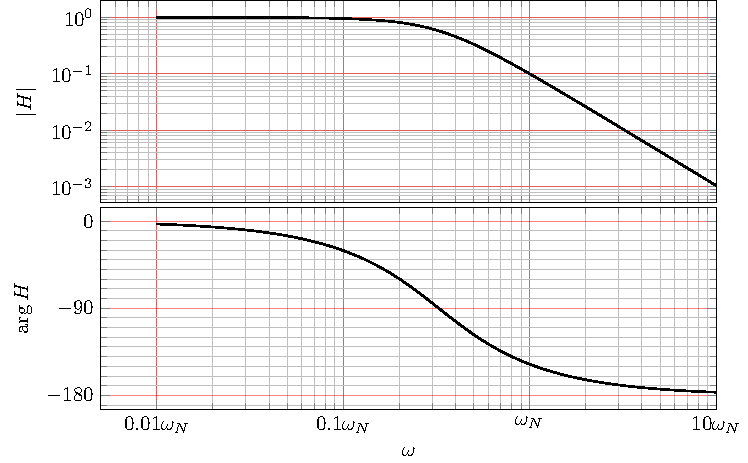
\includegraphics[width=0.8\linewidth]{../../figures/ps7-bessel-bode}
\end{center}

\begin{enumerate}
\item What is the bandwidth of the filter?
\item Determine the filter parameter \(\omega_0\) in terms of \(\omega_N\).
\item What is the phase shift at the Nyquist frequency?
\item Assume that the cross-over frequency of the loop gain is \(\omega_c = 0.1\omega_N\). What is the phase shift at this frequency?
\item What delay $T$  does this correspond to if the filter is approximated as a pure delay \(H(i\omega) \approx \mexp{-i\omega T}\)?
\item How large is the delay in terms of the sampling period \(h = \frac{\pi}{\omega_N}\)?
\end{enumerate}


\section*{Choice of bandwidth of antialiasing filter}
\label{sec-2}

\begin{center}
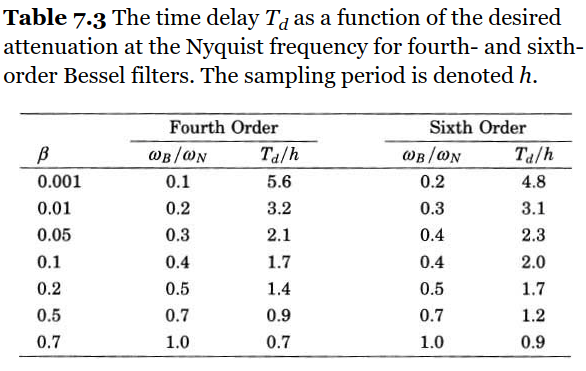
\includegraphics[width=0.4\linewidth]{../../figures/Astrom-fig73.png}
\end{center}
The table can be used to find the delay in the feedback path caused by an antialiasing filter. For instance, if we want to have an attenuation at the Nyquist frequency equal to \(\beta = 0.01\), then a fourth-order Bessel low-pass filter will give a delay of about \(T_d = 3.2 h\), that is a delay of more than 3 sampling periods. 
\begin{enumerate}
\item What is the advantage of using an antialiasing filter of higher order than 2?
\item If we can only accept a time delay of maximum two sampling periods, what is the attenutation we can obtain at the Nyquist frequency?
\item If the bandwith frequency of the antialiasing filter is chosen equal to the Nyquist frequency, \(\omega_B = \omega_N\), then by definition of the bandwidth of a filter we have that the attenuation at \(\omega_N\) is 0.7=-3dB. If the sampling period is 0.4 seconds. What is the time delay due to a sixth-order antialiasing filter?
\item What is the attenuation of a forth-order filter at \(5\omega_B\)
\end{enumerate}

\section*{Discuss choice of sampling frequency and antialiasing filter}
\label{sec-3}
A continuous-time signal $f(t)$ with the Fourier transform $F(\omega)$ given below is to be sampled for the purpose of feedback control. It is known that the signal is corrupted by noise in the form of a sinusoid of frequency $5\omega_0$.

\textbf{Discuss the choice of sampling frequency and antialiasing filter}

Hints: 
\begin{itemize}
\item There are two alternatives: With antialiasing filter, with no antialiasing filter, but digital low-pass filtering.
\item When sampling, the frequencies are "folded" at the Nyquist frequency.
\end{itemize}

\begin{center}
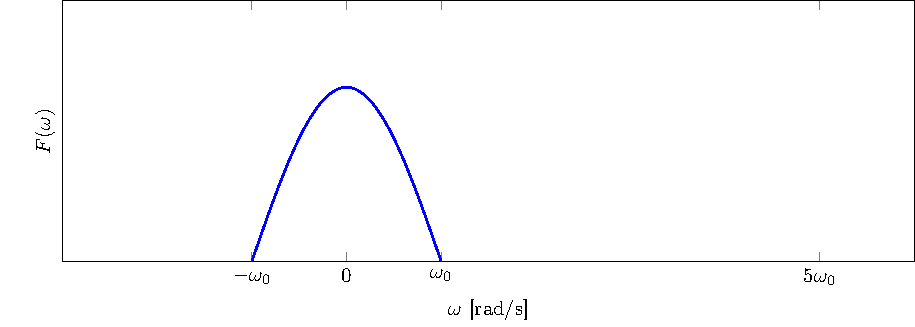
\includegraphics[width=0.7\linewidth]{../../figures/choose-sampling-frequency}
\end{center}
% Emacs 25.3.50.2 (Org mode 8.2.10)
\end{document}